%!TEX root = DMmidterm.tex

\section{Project}
\label{sec:Project}

%\begin{figure*}[]
%	\begin{center}
%		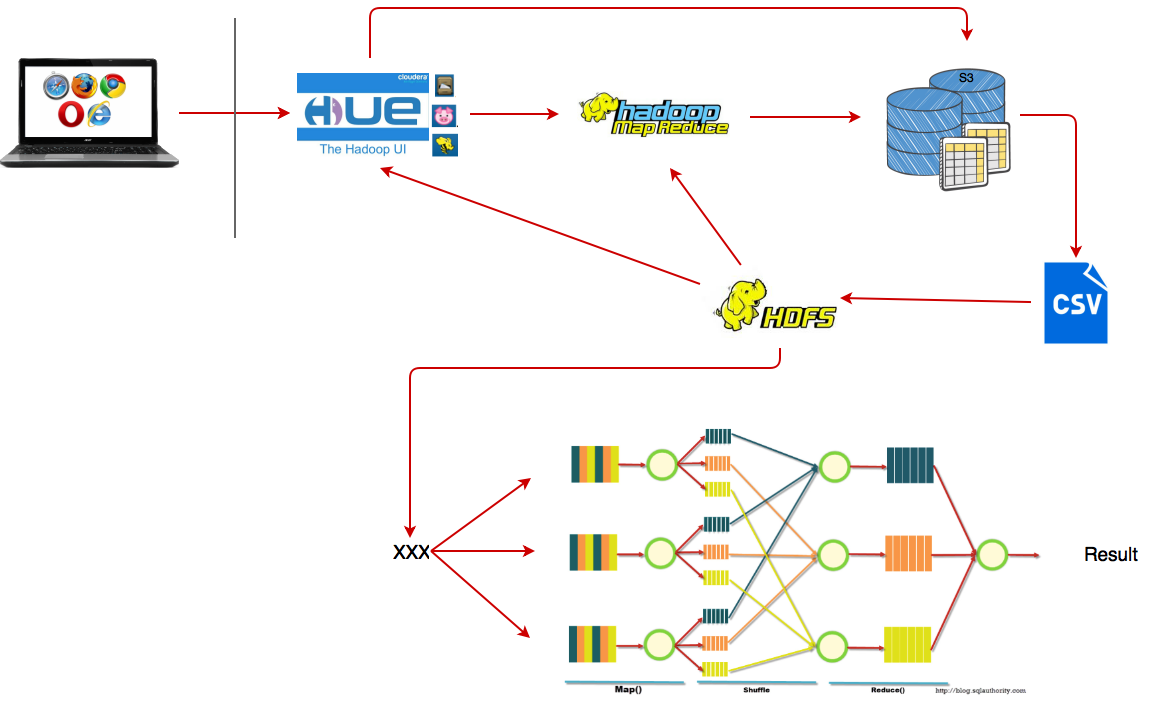
\includegraphics[width=2\columnwidth]{/Users/MariaFerman/Desktop/DC_FinalProject/images/Diagram}
%		\caption{Project Diagram}
%		\label{fig:dataDiagr}
%	\end{center}
%	\vspace{-10pt}
%\end{figure*}

%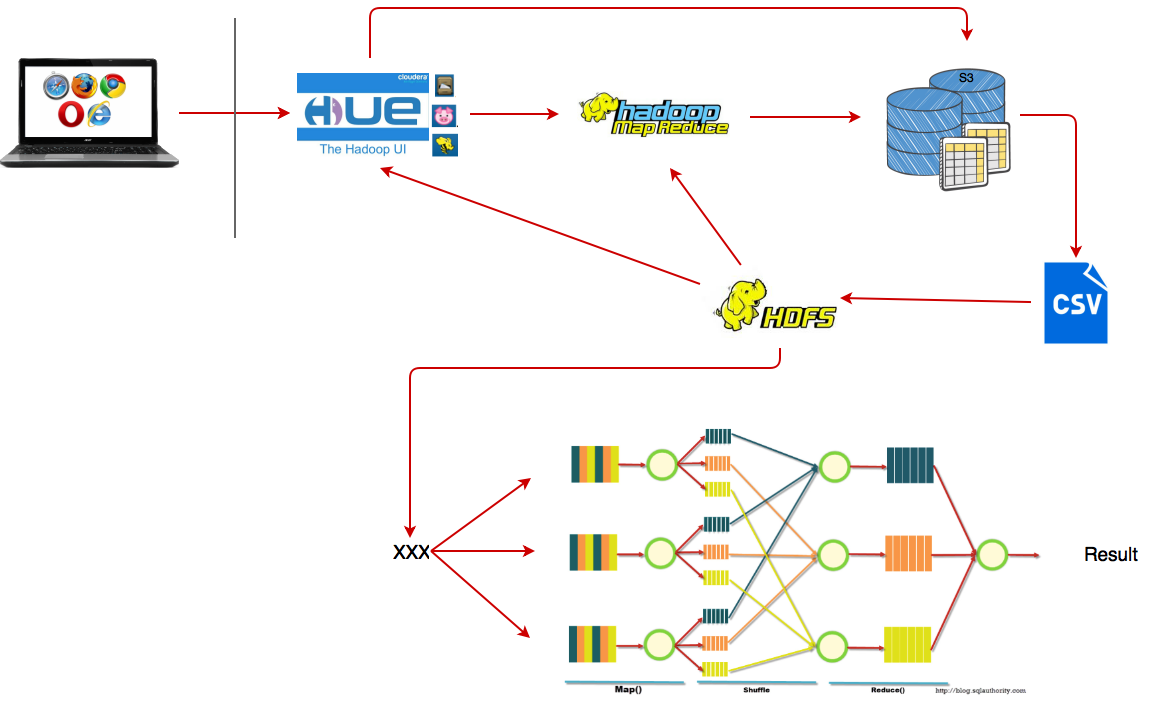
\includegraphics{/Users/MariaFerman/Desktop/DC_FinalProject/images/Diagram}


\subsection{ Dataset}
The dataset gathered for this project comes from the Pacific Climate Impacts Consortium (PCIC) of the University of Victoria. The dataset consist in a series of climate measurements that shows how the climate changes and varies over time. All the measurements were gathered at the same location in the Pacific and Yukon region of British Colombia, Canada.
%The dataset has different networks such as BC Hydro,  environmet Canada, Ministry of transportation among other. 
The dataset is divided by time and stations. The station is the exact location where the data were gathered. 
The dataset will allow us to understand the climate change among time and regions (stations). The resulting analysis of the dataset might help for trend analysis and climate change researches. This information can be used as an input for more complex climate models in order to have accurate climate predictions.

\subsection{Scripts}
The project implementation begins by using two customised scripts for the Hive and Pig process, the first script is for getting the data and the second is for storing and doing some computations. 
\subsubsection*{Pig script} To add ...
\subsubsection*{Hive script}
This script uses sql command for selecting the data form the Hadoop Distributed File System. The script only select the require information for doing the posterior computations for analyzing of the data. 
\begin{lstlisting}
SELECT ds562.time, ds562.one_day_precipitation, ds562.max_temp, ds562.min_temp 
FROM ds562
\end{lstlisting}

\subsection{Implementation}
We setup a EMR cluster on Amazon Web Service.
The cluster is consist of 3 nodes, 1 mater and 2 core(workersw). All nodes are running Lastest Ubuntu as its operating system while installed Hadoop, Hue, Hive and Pig by default.
Hue is stalled on master node while the other 3 are achitectures involved both master and core nodes.
So we do not need to do extra configuration or application installation for our data analysis.
The raw climate data are uploaded onto S3. And all output and logs are also stored in S3.
The archtecure of the system are shown in fig1 and fig 2. fig1 shows the data process path of Pig while fig2 shows the data process path of Hive.
We use Pig to load raw data from S3, and then caculate the average values of each columns and stored them in HDFS format.
After the processed data are in HDFS, we can use Hive which provides SQL executor to access the data.
Hue is a web page that providing interface for Pig and Hive. 

\begin{figure}[h!]
	\begin{center}
		\includegraphics[width=1\columnwidth]{../images/PigDiagram}
		\caption{Pig Diagram}
		\label{fig:dataDiagr}
	\end{center}
	\vspace{-10pt}
\end{figure}


\begin{figure}[h!]
	\begin{center}
		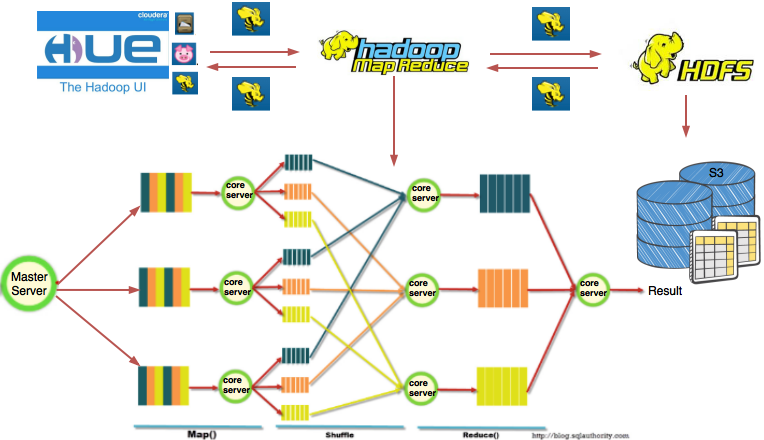
\includegraphics[width=1\columnwidth]{../images/HiveDiagram-2}
		\caption{Hive Diagram}
		\label{fig:dataDiagr}
	\end{center}
	\vspace{-10pt}
\end{figure}


